% !TEX encoding = UTF-8 Unicode
%!TEX root = ../Main/thesis.tex
% !TEX spellcheck = en-US
%%=========================================
\documentclass[../Main/thesis.tex]{subfiles}
\begin{document}
	\chapter[Conclusions]{Conclusion}
	\label{sec:conclusions}
	 In section \ref{sec:comp}, the results obtained from the high frequency resonance technique and the scheme presented in this thesis are compared.
	 Section \ref{sec:summary_and_conclusions} gives a summary, followed by a discussion regarding the main results, and recommendations to extend this work.

	
	%%=========================================
	\section{Comparison of results}
		\label{sec:comp}
	Figure \ref{fig:hfrt-method} and \ref{fig:yapi-method} show the frequency spectrum obtained from the high frequency resonance technique (HFRT), and the method proposed in this thesis, respectively. The magnitude of each peak in the spectrum given by the HFRT is in G or $mm/s^{2}$. Whereas, the magnitude of the peaks obtained in this thesis are in energy square per Hertz. That is, the energy contribution per Hertz. Regardless, for bearing fault detection, a high magnitude defect frequency, corresponds to a severe bearing fault. 
	\justify
	 Both Figures represent the spectrum of a signal obtained from a bearing with an inner ring defect. The latter can produce a noisy frequency spectrum when the HFRT is applied. This can been seen from Figure \ref{fig:hfrt-method}, which shows a relatively noisy frequency spectrum.
	Although the HFRT applies a series of filtering in order to strip out irrelevant signal components, the resulting frequency spectrum still contains  peaks embedded in noise. Consequently, identifying bearing faults with certainty, can be challenging. 
	
	\begin{figure}[H]
		\centering
		%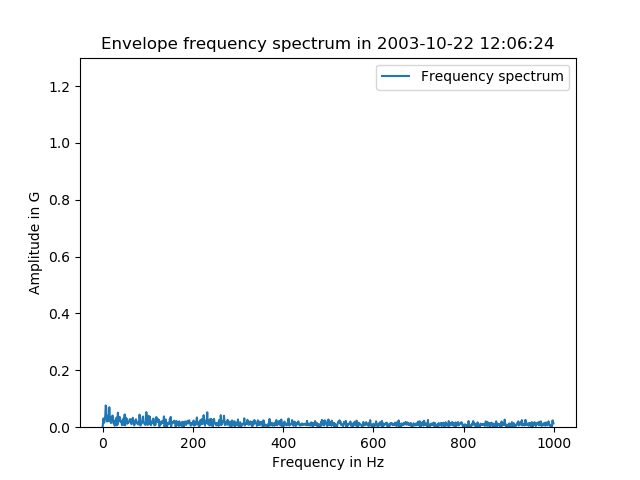
\includegraphics[width=0.7\linewidth]{../fig/bpfi/first_day_spectrum}
		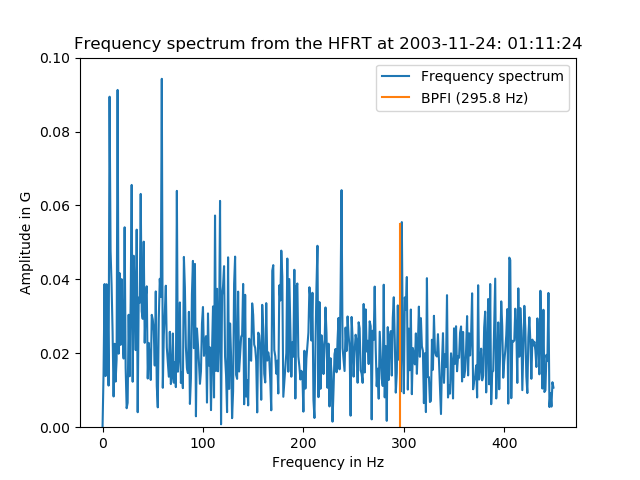
\includegraphics[width=0.7\linewidth]{../fig/hfrt}
		\caption{Frequency spectrum with an identified ball pass inner race defect frequency obtained from the high frequency resonance technique (HFRT).}
		\label{fig:hfrt-method}
		
		\begin{figure}[H]
			\centering
			%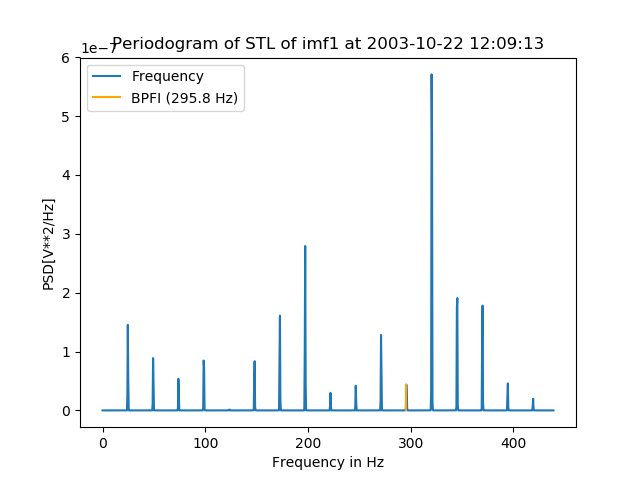
\includegraphics[width=0.8\linewidth]{../fig/periodogram_bpfi/start_imf1_bpfi}
			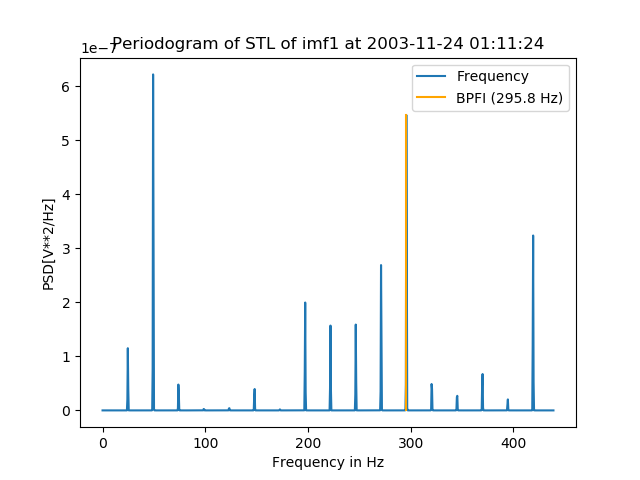
\includegraphics[width=0.7\linewidth]{../fig/periodogram_bpfi/end_imf1_bpfi}
			\caption{Frequency spectrum with an identified ball pass inner race defect frequency obtained from the method posited in this thesis.}
			\label{fig:yapi-method}
		\end{figure}
	\end{figure}
\justify
In contrast, Figure \ref{fig:yapi-method} shows a clear spectrum with conspicuous frequency peaks. By applying the empirical mode decomposition on the target vibration signal, the most relevant information is extracted. Furthermore, the seasonal component of the extracted intrinsic mode function represents a relatively noiseless signal. This means that only part of the signal containing diagnostic information are captured. With enough information of the machine, the origin of most peaks on the frequency spectrum could be (almost) explained. 
This make bearing fault diagnosis easier and accurate, as we are only restricted to few frequency peaks to analyze.

	\section{Summary}
	\label{sec:summary_and_conclusions}
	 The proclivity of machines towards failure, imposes a monitoring and maintenance scheme, in order to avoid unexpected and catastrophic breakdown. To mitigate such events, most machines are equipped with an array of sensors, collecting continuously data. By applying signal processing methods, incipient failures can be detected.
	\justify
	 Being continually subjected to extensive load and stress, bearing failures represent more than 40$\%$ of defects in rotating machines. In most industries, Fourier transform is the corner stone of nearly all methods, applied to bearing faults detection.
	One of the most widely used scheme is the high frequency resonance technique (HFRT). 
	The HFRT filters a bearing vibration signal, in order to remove noise, and isolate desirable components, before generating a frequency spectrum. For a bearing, the failure frequencies are derived from its geometrical components and the rotational speed of the machine on which it is mounted. Once the failure frequencies are available (given by the manufacturer), it suffices to search for them in the frequency spectrum, derived from the Fourier transform. 
	\justify
	The high frequency resonance technique although widely used, can produce a very noisy spectrum, in particular when the bearing is subjected to a severe inner race defect. This can render fault detection very challenging. In this thesis therefore, a new method is presented to mitigate this issue.
	This proposed scheme, consists of decomposing an input bearing vibration signal, into successive high to low frequency components called intrinsic mode functions (IMFs). This is achieved through the empirical mode decomposition (EMD).
	\justify
	Once the intrinsic mode functions (IMFs) have been computed, the first IMF is selected. Furthermore, its seasonal trend is computed through the seasonal trend decomposition method by LOESS (STL). The STL is a computational efficient method that decomposes a signal into its trend and seasonal part. The trend is a monotone function, while the seasonal part is a periodic oscillatory sinusoidal. Moreover, the power spectral density of the seasonal component of the first intrinsic mode function is approximated. This is achieved through the periodogram method (approximation of the power spectral density). 
	To test the efficiency of the proposed method, a case study was performed. The results show that the new technique was able to identify bearing failures. In addition, the frequency spectrum obtained was relatively noiseless, compared to the one computed through the high frequency resonance technique.
	\justify
	The Hilbert-Huang transform, through the empirical mode decomposition (EMD), boasts itself in generated mono component intrinsic mode functions. However, the EMD suffers from what is known as mode mixing. The latter introduces one or more oscillatory modes into an IMF. This is precisely the reason why in this thesis, the seasonal component of each IMF is extracted through the STL, in order to circumvent mode mixing.
	\justify
	The result obtained are satisfactory in the sens that, bearing failure frequencies are clearly identified. However, only two types of bearing failures were tested: namely faults occurring in the inner and outer ring. The justification is that these are the prevalent faults encountered. As an extension to this work, the new method could be applied to detecting the whole range of bearing defects, in order to further test its full validity. In addition, since the data for this case study was obtained under a control experiment, the new scheme could be tested with data from real industrial processes.

	
\end{document}
